\documentclass[11pt,a4paper]{article}
%\usepackage{harvard}
\usepackage[margin=1.5cm, bottom=2cm]{geometry}
\usepackage{graphicx}
\usepackage{tabularx}
\usepackage{color}
\usepackage{caption}
\usepackage{tabu}
\usepackage{gensymb}
\usepackage{enumitem}

\captionsetup[figure]{labelfont=bf}
\captionsetup[table]{labelfont=bf}

\title{\vspace{-2em}Virtual and Augmented Reality}
\author{pbqk24}
%\date{}

\begin{document}
	\maketitle
	
	\vspace{-3em}
	
	\section*{Problem 1}	
	The following functional interfaces were created:
	
	\begin{table}[h!]
		\caption{Functional interfaces implemented and their inputs/outputs}
		\label{table_functional_interfaces}
		\begin{tabu} to 1.0\linewidth {|X[l]|X[l]|X[l]|}
			\hline
			\textbf{Functional interface}&\textbf{Inputs}&\textbf{Outputs}\\
			\hline
			Euler angle $\rightarrow$ quaternion conversion&Euler angles in radians of format $(x, y, z)$&A quaternion of format $(w, x, y, z)$\\
			\hline
			Quaternion $\rightarrow$ Euler angle conversion&A quaternion of format $(w, x, y, z)$&Euler angles in radians of format $(x, y, z)$\\
			\hline
			Quaternion conjugate calculation&A quaternion of format $(w, x, y, z)$& The conjugate of the input: $(w, -x, -y, -z)$\\
			\hline
			Quaternion product calculation&Two quaternions $a, b$ of format $(w, x, y, z)$&The product of $a$ and $b$ of format $(w, x, y, z)$\\
			\hline
		\end{tabu}\\
	\end{table}

	\noindent Similar descriptions for each function are also included in the code.
	
	\section*{Problem 3}
	
	Several different alpha values were investigated for the tilt-corrected orientation tracking. They are listed in Table \ref{table_alpha_tilt} below, along with a description of the findings:
	
	\begin{table}[h!]
		\caption{Effect of Alpha Values on Drift Compensation in Tilt-Corrected Orientation Tracking}
		\label{table_alpha_tilt}
		\begin{tabu} to 1.0\linewidth {|r|X[l]|}
			\hline
			alpha&Description\\
			\hline
			$0.01$&Minimal change from simple dead reckoning filter. Slightly reduces the manifestation of gimbal lock in $X$ and $Y$ axes during the $-90\degree$ rotation around $Y$. $X$ and $Y$ rcomponents are marginally further from $0$ at the end of the sequence.\\
			\hline
			$0.03$&Slight increase in the manifestation of gimbal lock compared to an alpha of $0.01$. $X$ and $Y$ components converge marginally closer to $0$ than with an alpha of $0.01$ and in dead reckoning filter, although the change is extremely subtle.\\
			\hline
			$0.05$&Significantly reduced gimbal lock manifestation when $Y \simeq \pm90$. $X$, $Y$ and $Z$ all converge to $0$ at the end of the sequence, however the last rotation of $90\degree$ in $Z$ has decayed to $\sim45\degree$.\\
			\hline
			$0.10$&Complete decay of all angles to $0$ after $t\sim8s$. Before this the $90\degree$ rotation around $X$ occurs, which reaches $90\degree$ then quickly falls towards $0$, instead of staying $\sim90\degree$ for a few seconds as expected. The orientation tracking has completely failed, as the (imperfect) corrections introduced by the tilt correction completely overpower any actual rotations registered after the first few seconds. This effect becomes more extreme as alpha is further increased.\\
			\hline
		\end{tabu}
	\end{table}
	
	\noindent An alpha value of $0.03$ was chosen as the best value, as this causes the $X$ and $Y$ components to be closest to $0$ at the end of the sequence without decaying the tracking of any of the $\pm90\degree$ rotations.

	\section*{Problem 4}
	
	As for Problem 3 above, several alpha values were investigated for the yaw-corrected orientation tracking. They are listed in Table \ref{table_alpha_yaw} below, along with a description of the findings. All investigation was done with an alpha of $0.03$ for tilt-correction; the alpha listed below is specifically the alpha used for yaw-correction.
	
	\begin{table}[h!]
		\caption{Effect of Alpha Values on Drift Compensation in Yaw-Corrected Orientation Tracking}
		\label{table_alpha_yaw}
		\begin{tabu} to 1.0\linewidth {|r|X[l]|}
			\hline
			alpha&Description\\
			\hline
			$0.0001$&The $Z$ component is slightly closer to $0$ at the end of the sequence, but there is still significant drift present. Thus, the yaw correction being applied is not strong enough, and a higher alpha value should be used.\\
			\hline
			$0.0002$&At this alpha value the $Z$ component is reduced to 0 at the end of the sequence, without decaying the $90\degree$ rotations or causing any visible inconsistencies in the graph. This produces the best results of all alpha values investigated\\
			\hline
			$0.0005$&The yaw drift is over-compensated, resulting in a significant drift in the $Z$ component at the end of the sequence, reaching $\sim\frac{-\pi}{2}$. This decay of the $Z$ component is noticeable from the end of the $-90\degree$ rotation around $Y$ at $t\sim16s$.\\
			\hline
			$0.0010$&Similar results as with alpha $=0.0005$, but more extreme. The $Z$ rotation is decayed by $\sim\frac{-\pi}{2}$ from $t\sim16s$ to the end of the sequence.\\
			\hline
			$0.0100$&The decay of $\sim\frac{-\pi}{2}$ in the $Z$ compoent is constant starting from $t\sim2s$. Significant noise is present in the $Z$ rotation, making it rapidly `jitter.'\\
			\hline
			$0.1000$&The $Z$ rotation shows the same general shape as for alpha $=0.01$, but the amount of noise is significantly larger. There are also occasional jumps from $-\pi$ to $+\pi$, for example when the headset is rotated by $-90\degree$ around the $Z$ axis.\\
			\hline
		\end{tabu}
	\end{table}
	
	\noindent An alpha value of $0.0002$ was chosen as the best value, as this caused the $Z$ component to converge with $X$ and $Y$ at $0$ at the end of the sequence. Additionally, with this alpha there is no noticeable distortion or over-correction at any point during the sequence.
	
	\section*{Problem 5}
	
	Note: the 3D plots produced for Problems 5 and 6 skip data points in order to render in the requested full-speed and half-speed. For full-speed, only every 25\textsuperscript{th} orientation is plotted, while for half-speed every 12\textsuperscript{th} orientation is plotted (these were the highest resolutions that worked for these speed constraints on my laptop). This is due to the rendering capabilities of Matplotlib, and the speeds may vary slightly depending on your hardware.
	
	\begin{figure}[h!]
		\centering
		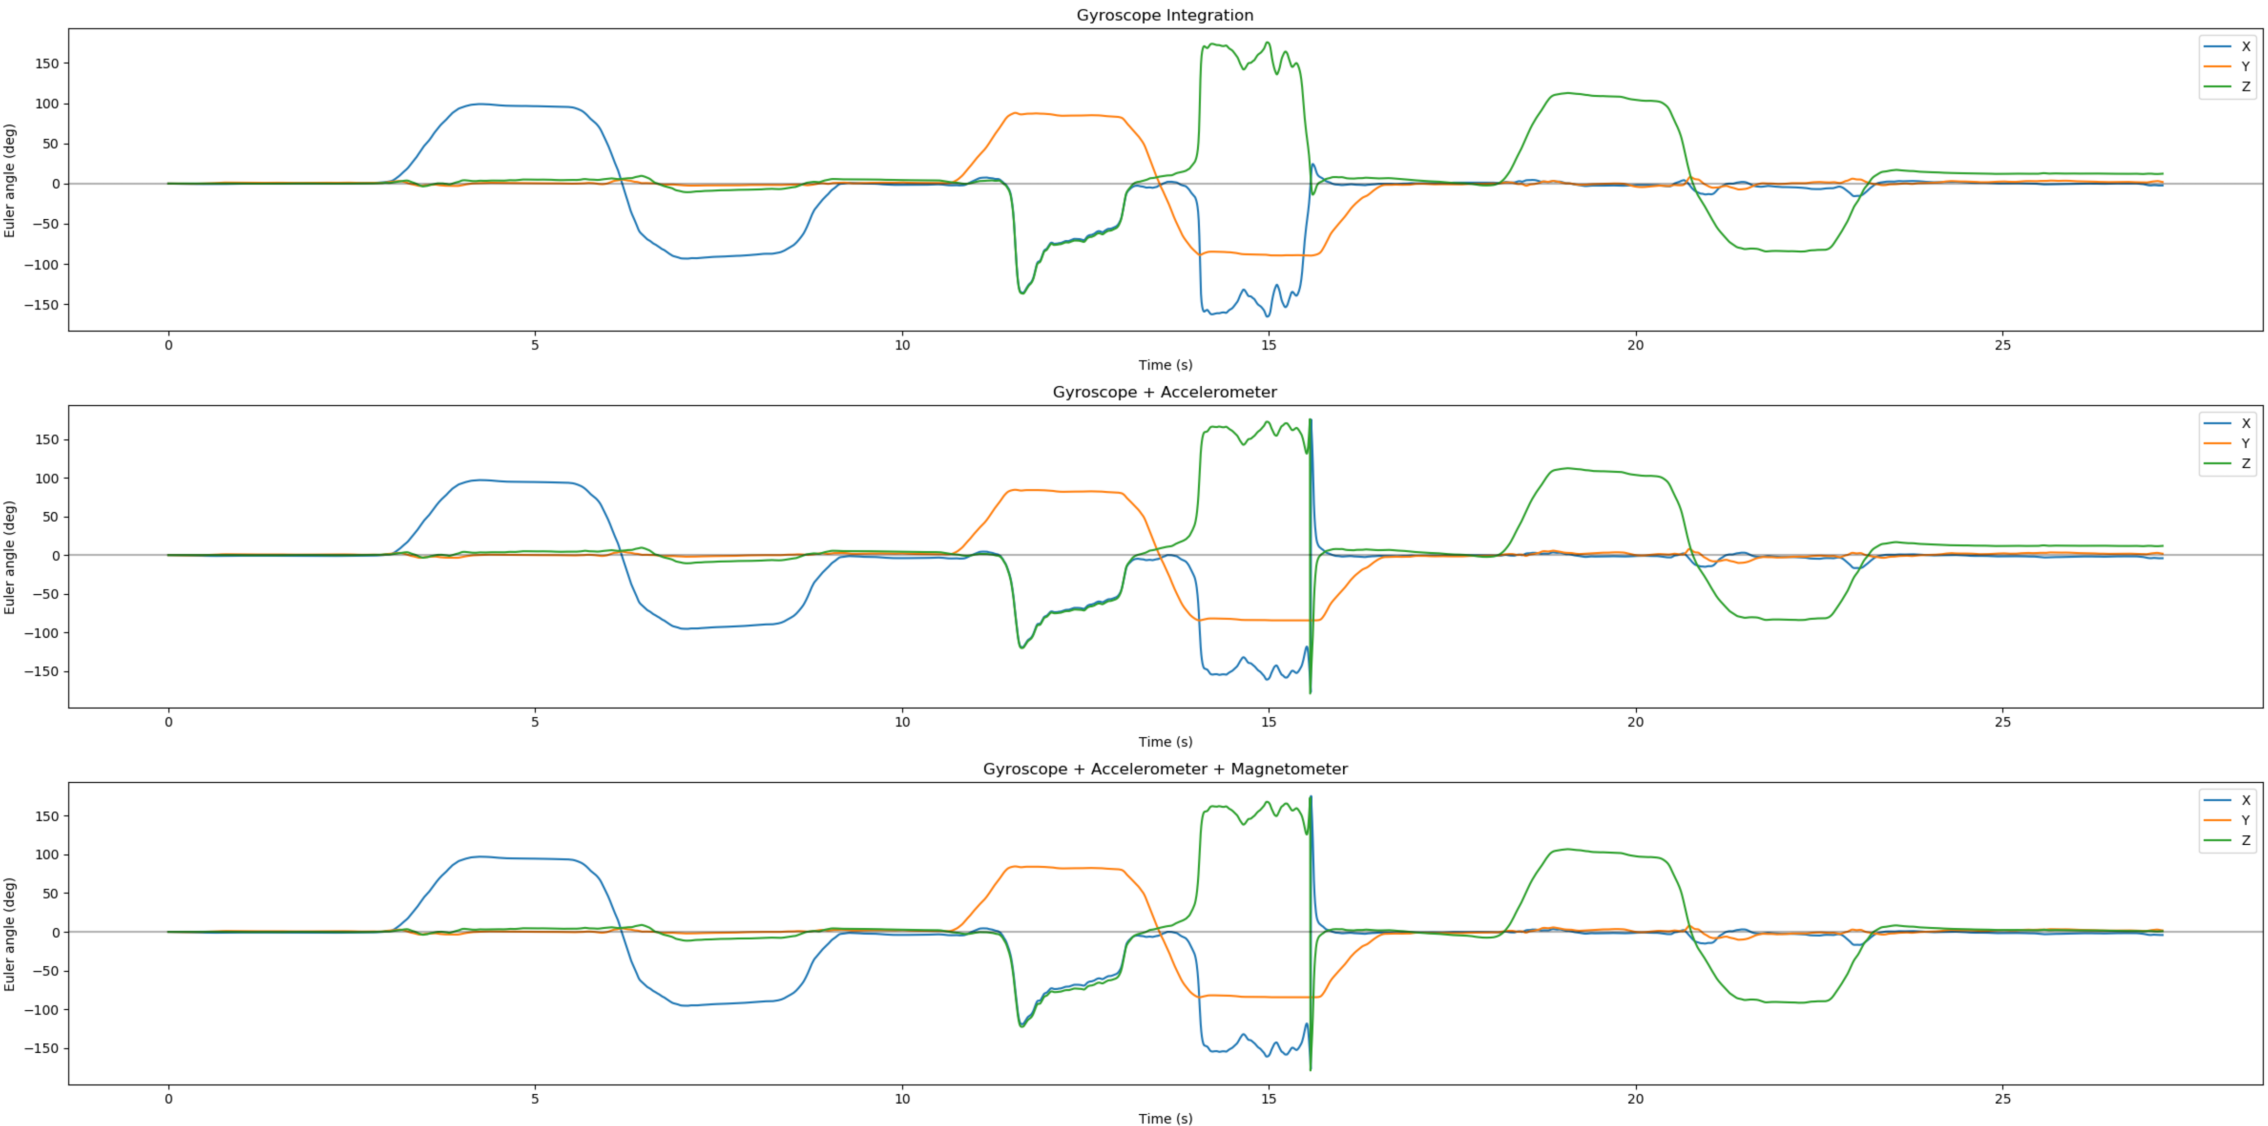
\includegraphics[width=1.0\linewidth]{figures/Orientation_Tracking_2D}
		\caption{2D Visualization of Various Methods for Head Orientation Tracking}
		\label{2D_Orientation}
	\end{figure}
	
	Figure \ref{2D_Orientation} show 2D plots of the results of head orientation tracking for the three different methods: simple dead reckoning (gyroscope integration), tilt correction (gyroscope + accelerometer), yaw correction (gyroscope + accelerometer + magnetometer). The $x$ axis represents time in seconds, and the $y$ axis of each plot represents the Euler angle for each axis in degrees, where $Z$ is vertical (the axis of yaw), $Y$ is horizontal (the axis of pitch), and $X$ is depth (the axis of roll).
	
	The simple dead reckoning and tilt-corrected orientation tracking approaches produce very similar results. Because the simple dead reckoning suffers from very little drift in the $X$ and $Y$ axes, there is little change once this drift is corrected for. The tilt correction does slightly improve the results however.
	
	As expected, the most stable method is the yaw-corrected head orientation tracking. This can be clearly seen by looking at the $Z$ component values at the end of the sequences. In both the simple dead reckoning and tilt-corrected orientation tracking approaches the $Z$ component suffers from gyroscopic drift, which is successfully corrected for by the yaw correction.
	
	This can also be clearly seen in the 3D plot shown in Figure \ref{3D_Orientation}. This is a snapshot from the end of the sequence of rotations, and thus the gyroscopic drift is relatively high. In this image both the simple dead reckoning and tilt correction suffer from yaw drift, while the yaw corrected tracking does not (most noticeable when comparing the $Y$ component vectors). This further showcases the improved stability of orientation tracking achieved by yaw correction.
	
	\begin{figure}[h!]
		\centering
		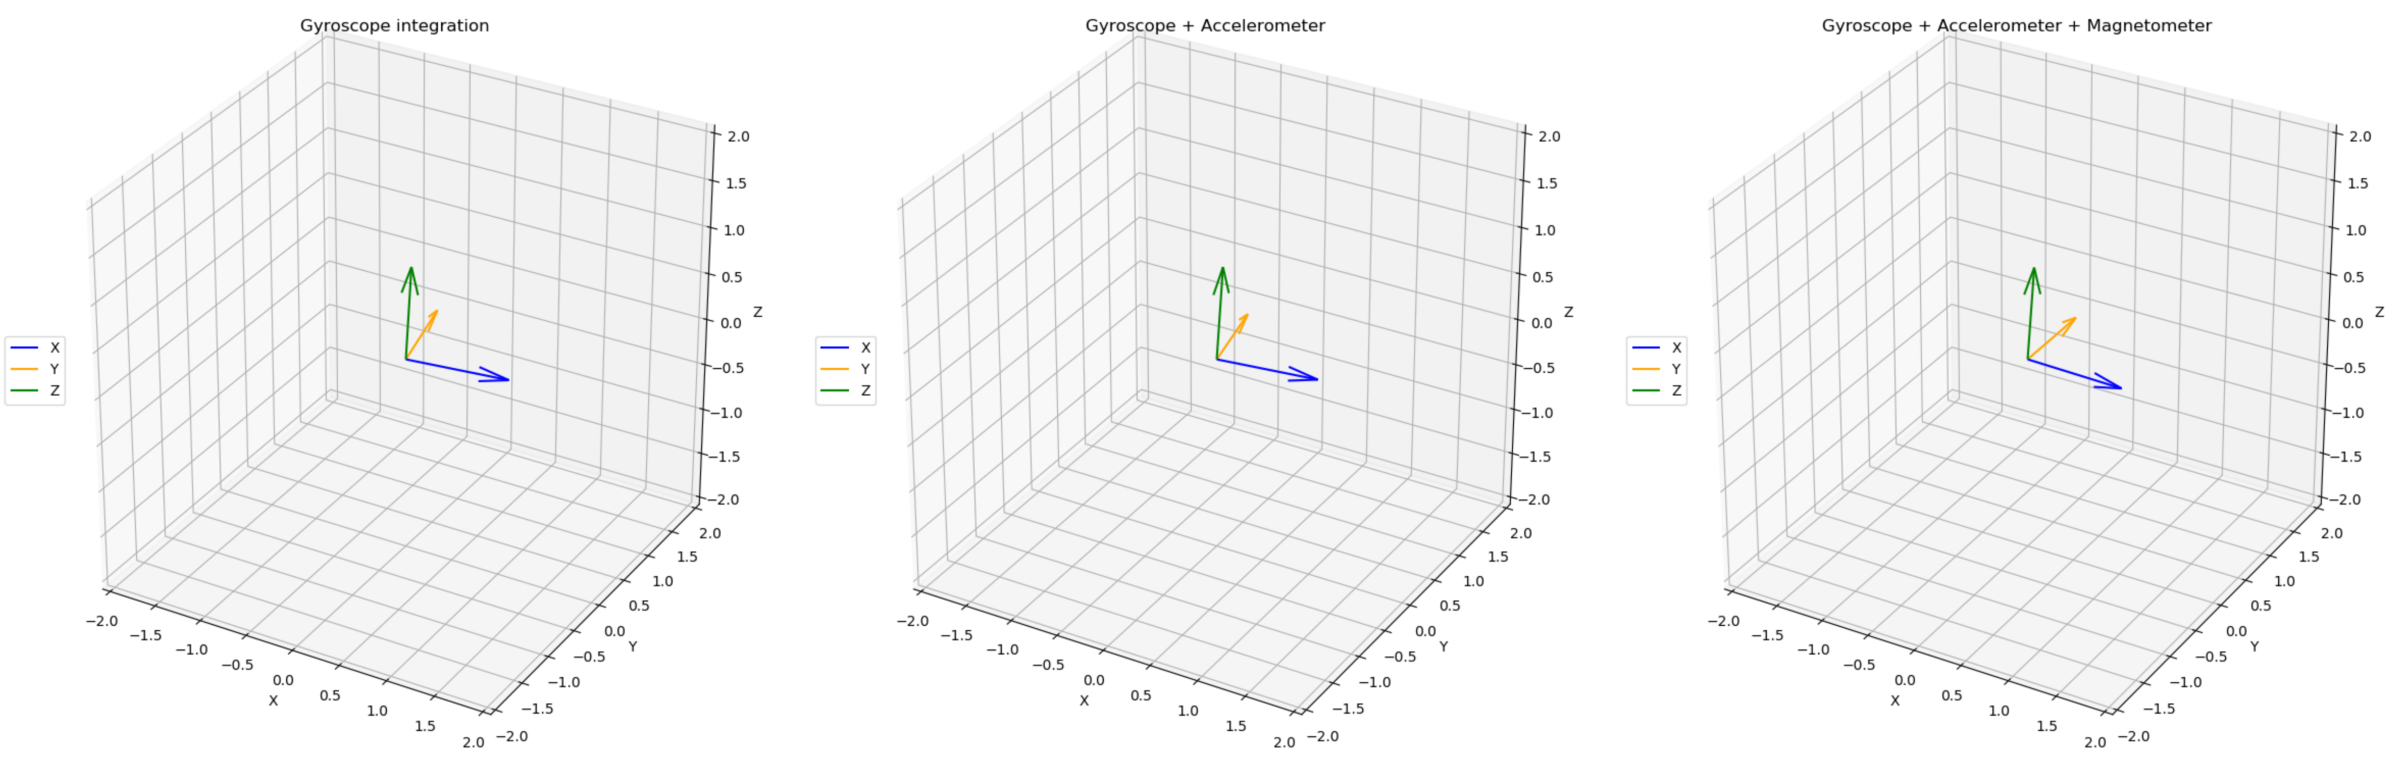
\includegraphics[width=1.0\linewidth]{figures/Orientation_Tracking_3D}
		\caption{Example 3D Result of Head Orientation Tracking}
		\label{3D_Orientation}
	\end{figure}
	
	
	\section*{Problem 6}
	
	In order to try to achieve positional tracking using the IMU, I double integrated the accelerometer readings and applied a two-bar kinematic head model. This assumes that the head is locked to the neck, the neck can be rotated about its base (at the joint to the torso), and the torso can be rotated around the waist. This was applied as follows:
	
	\begin{enumerate}[noitemsep]
		\item Convert acceleration readings to global acceleration by rotating the readings by the current head orientation estimate: $a_{global}=q*(0, a_x, a_y, a_z)*q^{-1}$
		\item Extract linear acceleration by subtracting gravity (1) from the $Z$ component
		\item Integrate the linear acceleration into velocity and convert into angular velocity as $\omega=\frac{a_l*\Delta t}{l_t}$, where $a_l$ is linear acceleration, $\Delta t$ is the time since the last time step, and $l_t$ is an estimated length of the torso, e.g. $l_t=0.8m$.
		\textbf{Note:} this makes the assumption that the linear acceleration is caused by a rotation of the body, rather than the neck and body combined
		\item Add the previous angular velocity reading to produce the current angular velocity
		\item Apply the simple dead reckoning filter to get an estimate for the orientation of the torso, $q_1$
		\item Calculate the position of the torso relative to the origin (the waist) as $r_1=q_1*(0,0,l_t)*q_1^{-1}$
		\item Apply the simple kinematic head model to get the position of the head relative to the torso, $r$, as $r=q*(0,0,l_n)*q^{-1}$, where $l_n$ is the estimated length of the neck, e.g. $l_n=0.15m$, and $q$ is the current estimated head orientation
		\item Compose the two positions to get the global position of the head as $p=r_1+r$
	\end{enumerate}

	This approach constrains the position of the head to what could physically be reached by a person anchored at the waist, such as when sitting down. Even with these constraints and the short duration of the data sequence (around 28s) there is significant drift in the positional tracking. One example of this is shown in Figure \ref{Position_Y_Rotation}. This shows a snapshot of the head position tracking for all three methods of orientation tracking, shortly after the $+90\degree$ rotation about the $Y$ axis ($t\sim12s$). In this image the gyroscope integration based method shows some drift in the $X$ and $Y$ components, and very high drift in $Z$ (see also Figure \ref{Position_2D}). The other tracking methods show slight drift, as they have a lower $X$ position than would be expected, but fare much better than the gyroscope integration. This is likely due to the poor performance of the gyroscope integration orientation tracking resulting in much larger errors due to the quadratic growth of drift error.
	
	\begin{figure}[h!]
		\centering
		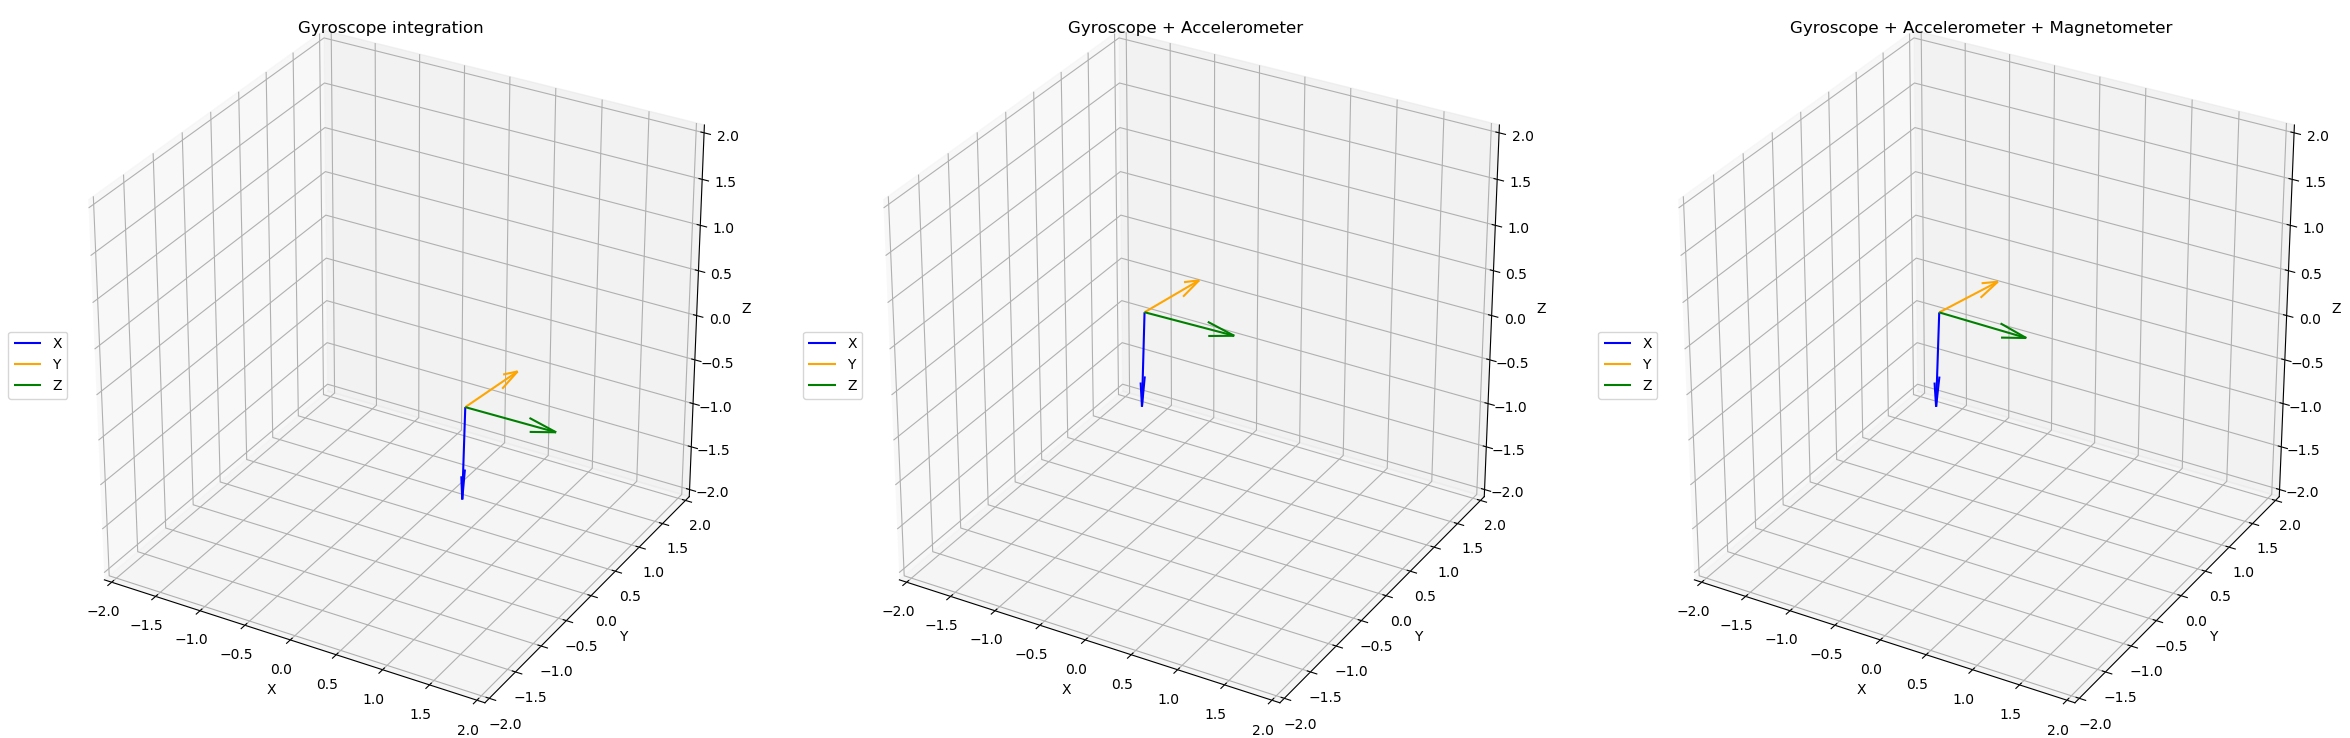
\includegraphics[width=1.0\linewidth]{figures/Position_Tracking_First_Y_Rotation}
		\caption{Example 3D Result of Various Methods for Head Orientation Tracking}
		\label{Position_Y_Rotation}
	\end{figure}

	Figure \ref{Position_2D} shows the tri-axial position tracking output for the three types of tracking. The left image shows gyroscopic integration position tracking. The right image shows tilt-corrected and yaw-corrected tracking, which produced extremely similar results. The gyroscope results are vaguely similar to the other methods until $t\sim5s$, where the positions all enter sinusoidal patterns. This obviously incorrect, and such tracking would likely make a user of the system ill very quickly. As previously mentioned, this drastic difference in positional tracking performance is likely caused by the poor performance of gyroscopic integration for orientation tracking, and the compounding of errors amplified by integration which are not corrected for.
	
	\begin{figure}[h!]
		\centering
		\begin{minipage}{0.45\linewidth}
			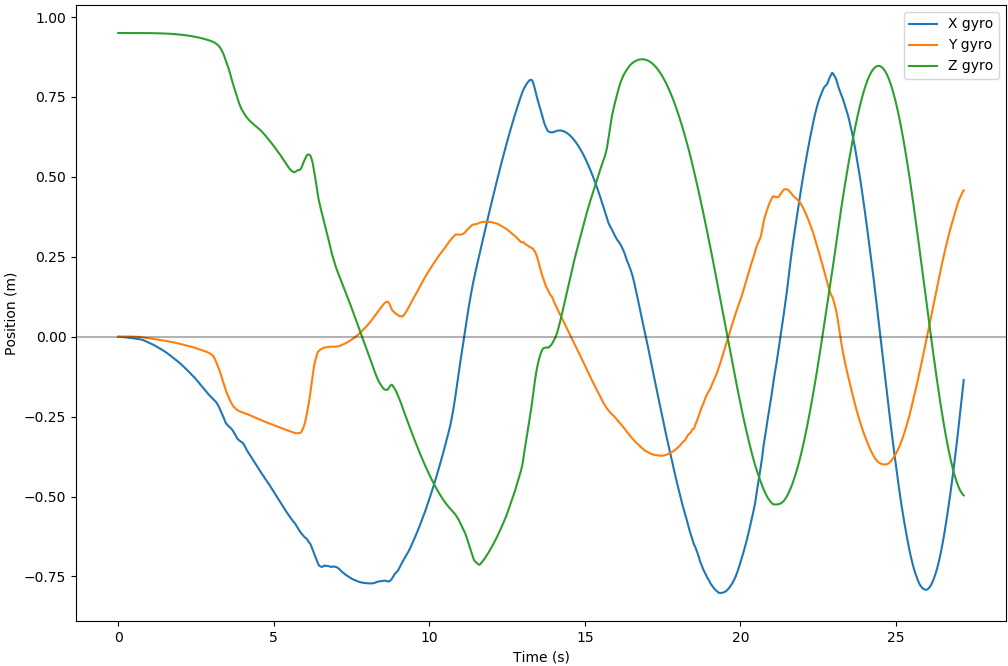
\includegraphics[width=0.9\linewidth]{figures/Position_Tracking_2D_Gyro}
		\end{minipage}		
		\begin{minipage}{0.45\linewidth}
			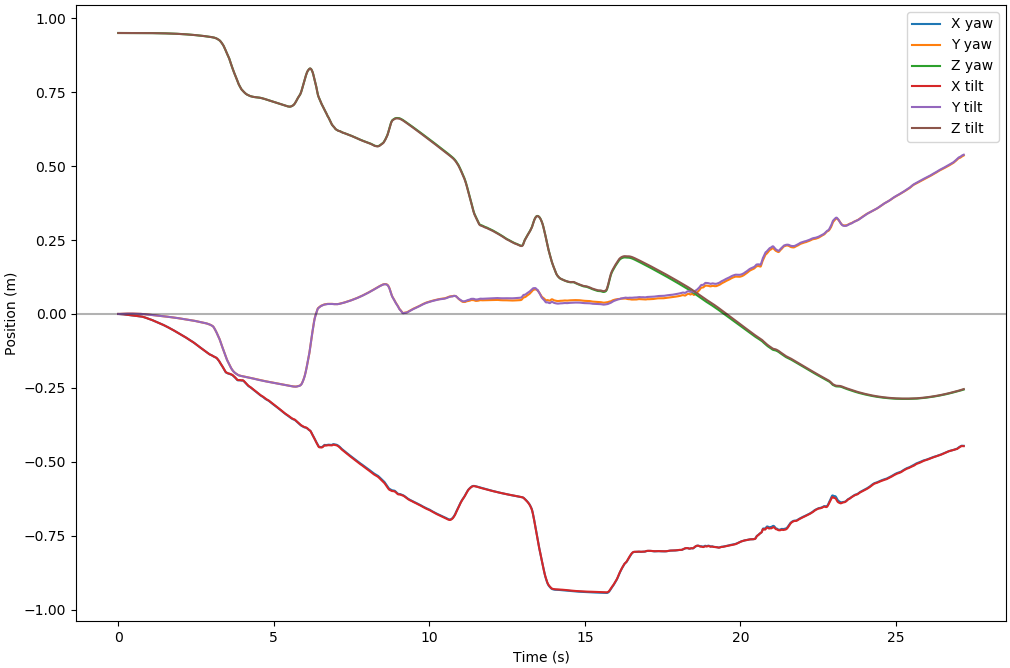
\includegraphics[width=0.9\linewidth]{figures/Position_Tracking_2D_Yaw_Tilt}
		\end{minipage}
		\caption{Example 3D Result of Various Methods for Head Orientation Tracking}
		\label{Position_2D}
	\end{figure}

	All methods of orientation tracking show significant drift in all three axes in positional tracking. This is likely caused by two main factors. Firstly, there is the large assumption made that the linear acceleration corresponds to rotation of the torso about the waist, rather than the neck around the base of the neck (or likely a combination of the two). This assumption was made in order to simplify the kinematic system, and justified by the fact that the neck often only slightly moves around its base, and most of the movement of the head relative to the waist is due to a rotation of the torso. Secondly, a large amount of error is introduced by the double integration of the accelerometer readings. Numerical integration by itself produces inaccurate results, and this is only made worse by applying double integration to already noisy data (as the accelerometer itself has inherent noise, and the local to global frame conversion is based on an imperfect head orientation estimate). All these sources of noise compound to produce potentially massive errors in the result, which are propagated in each time step of the tracking. Thus, any positional tracking based only on the IMU with no external frame of reference is going suffer from large drift and propagated errors.
\end{document}